\chapter{Detalles de Implementación y Experimentos}\label{chapter:implementation}
Para poder valorar la viabilidad de la propuesta realizada en este trabajo, es
necesaria la implementación de un prototipo del modelo explicado en el capítulo
anterior.


\section{Herramientas y tecnologías utilizadas}\label{section:implementation:techs}
\subsection{Lenguaje de programación Python}
Python es un lenguaje de programación de propósito general y alto nivel desarrollado por Guido van Rossum en 1991. Su filosofía de diseño enfatiza la legibilidad del código con el uso de sangría significativa. Python se tipifica dinámicamente y tiene incorporado un recolector de basura. Admite múltiples paradigmas de programación, incluida la programación estructurada, orientada a objetos y funcional. La más reciente  versión liberada al momento de realizarse este trabajo es la 3.11 [\cite{python_executive_summary_2022}].

Es altamente empleado para ingeniería y análisis de datos, aprendizaje de máquina
e inteligencia artificial gracias a sus vasta cantidad de bibliotecas como NumPy, Tensorflow, Keras, Pytorch, SciPy, Pandas y Matplotlib, entre otras creadas tanto por el mismo equipo de trabajo de Python como la propia comunidad. Para desarrollo web cuenta con marcos de trabajo (frameworks) como Django. Es altamente utilizado en la educación al ser de fácil aprendizaje y asimilación logrando así reducir la barrera de entrada al mundo de la programación a todo aquel interesado.

 En la actualidad sigue manteniendo el primer puesto de los índices de TIOBE y PYPL ratificando el interés de gran parte de la población y de los empleadores por este lenguaje y las ventajas que ofrece. Grandes organizaciones como Google [\cite{quotes_about_python_2021}], el CERN [\cite{python_the_holy_grail_of_programming_2014}], la NASA [\cite{python_success_stories_2021}], Yahoo [\cite{organizationsusingpython}], Wikipedia, Amazon, Facebook, Instagram [\cite{meta_for_developers_2018}], Spotify, entre otros.
Para este trabajo se utilizó la versión 3.7 para lograr una retro-compatibilidad
alta.

\subsubsection{numpy}
Constituye una biblioteca de Python de código abierto, la cual permite generar, tanto vectores como matrices, de grandes dimensiones y operar de manera cómoda y sencilla con ellos [\cite{numpy_2012}].
Consigue esto gracias a que utiliza internamente el lenguaje C para lograr efectuar de forma rápida operaciones muy costosas entre elevadas dimensiones.
En las etapas posteriores a la limpiezas de los datos explicada en el capítulo anterior se utiliza Numpy para el trabajo con los datos.

\subsubsection{matplotlib}
Matplotlib es una biblioteca de gráficos creada en 2003 por John D. Hunter para el lenguaje de programación Python y su extensión matemática numérica NumPy. Proporciona una API orientada a objetos para incrustar gráficos en aplicaciones utilizando kits de herramientas GUI de uso general como Tkinter, wxPython, Qt o GTK.
Es una biblioteca completa para crear visualizaciones estáticas, animadas e interactivas. Matplotlib hace que las cosas fáciles, pues sigan siendo fáciles y las difíciles sean posibles, como lo es crear gráficos con calidad de una publicación y hacer figuras interactivas que puedan hacer zoom, desplazarse, actualizar.

\subsubsection{scipy}
SciPy es una biblioteca de Python gratuita y de código abierto que se utiliza para la computación científica y la informática técnica. SciPy contiene módulos para optimización, álgebra lineal, integración, interpolación, funciones especiales, FFT (Transformada Rápida de Fourier), procesamiento de señales e imágenes, solucionadores de ODE (Ecuaciones Diferenciales Ordinarias) y otras tareas comunes en ciencia e ingeniería. Esta creada encima de la biblioteca Numpy anteriormente mencionada y fue desarrollada por la compañía Enthought en el año 2001.


\subsubsection{boto3}
Se utiliza el Kit de desarrollador de software (SDK por sus siglas en inglés) de AWS (Servicios Web de Amazon) para Python (Boto3) para crear, configurar y administrar servicios de AWS, como Amazon Elastic Compute Cloud (Amazon EC2) y Amazon Simple Storage Service (Amazon S3). El SDK proporciona una API (Interfaz para Programas de Aplicación) orientada a objetos, así como acceso de bajo nivel a los servicios de AWS.

Este SDK es empleado para acceder a los datos.

\subsubsection{pathlib}
Este es un módulo de Python que ofrece clases que representan rutas de sistemas de archivos con semántica apropiada para diferentes sistemas operativos. Las clases de ruta se dividen entre rutas puras, que proporcionan operaciones puramente computacionales sin Entrada/Salida (I/O por sus siglas en inglés), y rutas concretas, que heredan de rutas puras pero también proporcionan operaciones de I/O.

La clase \textit{Path} de esta biblioteca es ampliamente usada en este trabajo.

\subsubsection{json}
Python tiene el módulo \textit{json} incorporado, que nos permite trabajar con datos JSON (Notación de objetos JavaScript).
JSON es un formato de archivo estándar abierto y un formato de intercambio de datos que utiliza texto legible por humanos para almacenar y transmitir objetos de datos que consisten en matrices y pares de atributos y valores. Es un formato de datos común con diversos usos en el intercambio electrónico de datos, incluido el de las aplicaciones web con servidores.

\subsubsection{mediapipe}
Desarrollada por Google \brackcite{mediapipe_2020}, Mediapipe es una biblioteca de código abierto la cual utiliza distintos tipos de modelos para solucionar de forma conjunta varios problemas de detección [véase Fig \ref{fig:mediapipe}]. De los modelos presentes en la biblioteca de Mediapipe solo fue utilizado el modelo Holistic, el cual engloba a los modelos para la detección de manos (modelo Hands), detección facial (modelo Face Mesh) y pose corporal (modelo Pose) realizando la sincronización de estos de manera eficiente garantizando un buen resultado final.

Para este trabajo solo fue necesario el uso de los modelos Hands y Pose de Holistic.

\subsection{Google Colaboratory}

Google provee un servicio gratuito en el navegador el cual brinda, de manera temporal, recursos computacionales (CPU,TPU,GPU,RAM,HDD) mientras se haga uso activo de los mismos. En dicha plataforma se le permite al usuario escribir y ejecutar código Python en un entorno basado en Jupyter Notebook.Siendo así una herramienta ideal para el aprendizaje de máquinas, el análisis de datos y la educación al posibilitar que personas de pocos recursos puedan acceder de forma fácil a herramientas para el aprendizaje de máquina las cuales muchas de ellas ya vienen incluidas en el entorno o son muy  sencillas de instalar en el mismo.
Cabe destacar que además del plan gratuito que incluye CPU de última generación, 13 Gb de RAM y 110 Gb de almacenamiento, nos da la posibilidad de utilizar Google Drive para ampliar el almacenamiento y  varios planes de pago para aumentar la capacidad computacional del entorno.


\section{Implementación de un prototipo}
Para el desarrollo de los métodos que solucionan las problemáticas resueltas en el capitulo anterior, y concreticen la propuesta ofrecida, se decide utilizar varias clases para un mayor nivel de abstracción y posibilidad de generalización de lo métodos propuestos.

\subsection{Descargar datos y filtrado}
Auxiliándose de la biblioteca \textit{boto3} y \textit{json} fue posible recorrer los elementos disponibles en el almacenamiento de Gutiérrez-González\brackcite{leynier-lsc-2021} para, una vez descargados, filtrar los frames que son enteramente ceros y corregir alguna de las palabras mal escritas que se denotan como inexistentes. Luego se guarda todo el corpus en un archivo \textit{dataset.json} el cual al cargarlo nuevamente es utilizable como diccionario de forma instantánea. Todo este trabajo primario se realiza desde Google Colaboratory para poder conformar mejor el conjunto de datos.

\subsubsection{Extracción de los Datos}
Para la extracción de los datos se utilizó la biblioteca \textit{boto3} con acceso al almacenamiento en la nube donde se encontraban los datos.
Para ello se importa el método \textit{client} de \textit{boto3}, el cual es instanciado en la url donde se encuentra el conjunto de datos, además de las claves de acceso, las cuales por privacidad del dueño de las mismas se sustituyen por valores de ``X'' [véase Código \ref{code:s3client}]. 

\vspace{0.5cm}

\begin{lstlisting}[basicstyle=\tiny,language=Python, caption={Instanciar cliente s3}, label={code:s3client}]
from boto3 import client
s3_client = client(
    "s3",
    config=Config(
        signature_version="s3v4",
        retries={"max_attempts": 10},
        s3={"addressing_style": "path"},
    ),
    region_name="ams3",
    endpoint_url="https://ams3.digitaloceanspaces.com",
    aws_access_key_id="XXXXXXXXXXXXXXXX",
    aws_secret_access_key="XXXXXXXXXXXXXXXXXXXXXXXXXXXXX",
)
\end{lstlisting}

Una vez obtenido el cliente configurado se descargan los datos del mismo, conociéndose que se encuentran en el bucket ``lsc-corpus'', los de las señas aisladas, puesto que son los únicos datos con seguridad de la seña que corresponde a cada frase.

\vspace{0.5cm}

\begin{lstlisting}[basicstyle=\tiny,language=Python, caption={Descargar usando el cliente s3}, label={code:download_s3client}]
from pathlib import Path
root=Path("/content")
bucket="lsc-corpus"    
paginator = s3_client.get_paginator('list_objects_v2')
pages = paginator.paginate(Bucket=bucket)
for page in pages:
    for obj in page['Contents']:
        extension = obj['Key'].split('.')[-1]
        name=obj['Key'].split('.')[0]
        if extension  in ['json']:
		  drivepath=(root/f"tesis-generacion-lsc/{obj['Key']}").resolve()
  		  (drivepath/'..').resolve().mkdir(parents=True,exist_ok=True)
  		  drivepath.touch()
  		  s3_client.download_file(bucket,obj['Key'],str(drivepath))
\end{lstlisting}

Aquí se realiza un paginado para poder recorrer de manera adecuada  los elementos del bucket para luego chequear la extensión de los archivos contenidos en cada página [véase Código \ref{code:download_s3client}].
Se conocen previamente que los datos anotados de los puntos de interés estaban recogidos en archivos con extensión \textit{json} por cada frase. En la primera parte del código se importa la clase \textit{Path} de \textit{pathlib} para trabajar de manera rápida y efectiva con los directorios que se van creando.

\subsubsection{Limpieza de los datos}
Una vez ya se posean los archivos \textit{json} referentes a cada frase del corpus se pueden entonces cargarlos para limpiarlos y organizarlos en un dataset mejor estructurado donde estén todas las frases juntas.

En este código [véase Código \ref{code:load_and_clean}] se utilizan expresiones regulares para la limpieza de las llaves, ya que incurrían en faltas de ortografía, errores tipográficos y de copiado. Al no poseer una forma clara de rectificar las tildes faltantes se decidió dejar así dichas palabras y recomendar el uso de un algoritmo de similitud antes de indexar en el dataset creado.
La primera expresión elimina todo lo que esté entre paréntesis en las llaves, puesto que esto no aporta nada a la información semántica de los mismos. Luego se reemplaza todas las ``nn'' por una ``ñ'' 
, se eliminan los dígitos que hayan quedado de manera residual del primer método y todos los guiones entre palabras para que estén de manera individual.
\vspace{0.5cm}

\begin{lstlisting}[basicstyle=\tiny,language=Python, caption={Cargar los json y limpiar las llaves}, label={code:load_and_clean}]
import numpy as np
import json
import re
root_tesis = (root/f"tesis-generacion-lsc/").resolve()
cendsor_path = "cendsor-corpus/keypoints/"
wrong_words={ 'barsura':'basura',
              'insipido': 'insípido',
              'investar':'inventar',
              'ostion':'ostion',
              'panciencia':'paciencia',
              'sacapunta':'sacapuntas',
              'zapia':'zapya'}
word_poses_dict={}
for dirpath,dirnames,filenames in os.walk(root_tesis/cendsor_path):
  for filename in filenames:
    key,extension=filename.split('.')
	
	###########################
	# Limpieza de las llaves
	###########################
	
    key=re.sub(r"\s*\(.*\)","",key)
    key= key.replace("nn",'ñ')
    key=re.sub(r"\s?\d","",key)
    key = key.replace("-"," ") 
    if key in wrong_words.keys():
      key=wrong_words[key]
    
	###########################
	
    with open((root_tesis/cendsor_path/filename).resolve(), 'r', encoding='utf-8') as json_list:
      poseframes=np.array(json.load(json_list))
      json_list.close()
		
	  #######################################################
	  # Limpieza de los frames de los gestos que son 0
	  #######################################################
      filtro = [m!=0.0 for m in  np.mean(poseframes, axis=1)]
      
      poseframes=poseframes[filtro]

	  #########################################################
	  
      single_gesture = poseframes.tolist()
      try:
        word_poses_dict[key].append(single_gesture)
      except:
        word_poses_dict[key]=[single_gesture]      
\end{lstlisting}
En el caso de los gestos, existen en el corpus frames en los cuales los modelos no detectaban nada y por tanto estos devolvían (0,0,0) para todos los puntos de interés de ese frame. Por tanto, se hace uso de la biblioteca \textit{json} para cargar el archivo y de la biblioteca numpy para realizar la limpieza de una manera más cómoda y rápida.
Luego de obtener la máscara (filtro) con la información de los frames vacíos, simplemente se indexa en el arreglo numpy guardando su resultado como si fuera ahora el arreglo original.

Como información adicional, se guarda el diccionario tanto en la nube como en el directorio local para su mejor aprovechamiento y eliminar pasos extras a la hora de probar la propuesta.





%%%%%%%%%%%%%%%%%%%%%%%%%%%%
%
% MOSTRAR EVIDENCIA DE LA SOLUCION
% PUEDE SER EN EXPERIMENTOS TAMBIEN
%
%%%%%%%%%%%%%%%%%%%%%%%%%%%%


\subsection{Creación de las Clases}
En esta subsección se trataran de forma más específica las clases utilizadas en la implementación de la propuesta.

\subsubsection{Clase TokenLSC}

Una seña esta asociada a la clase \textit{TokenLSC}, la cual está conformada  por un nombre y una lista de Skeleton, los cuales no son más que una clase para abstraer conceptualmente un frame. La clase Skeleton cuenta con 3 Bodyparts para su inicialización, las cuales deben ser pasadas como argumentos a su constructor. Estas son la conceptualización de los puntos referentes a un tipo de parte del cuerpo, los cuales son representados mediante un enumerador (\textit{enum}) inicialmente.
La clase \textit{TokenLSC} cuenta con una serie de atributos y métodos para solventar de manera correcta los problemas planteados en el capitulo anterior, siendo estos métodos descritos a continuación, así como los correspondientes utilizados de Skeleton y Bodypart para ayudar a su cumplimiento.

La clase \textit{TokenLSC} esta conformada por un nombre (el cual hace referencia al identificador de la seña),  una lista de objetos de tipo Skeleton, los cuales a su vez están conformados  por 3 partes de cuerpo (son la clase Bodypart creada para este propósito). Además, al construirse la clase \textit{TokenLSC}, también se configuran valores necesarios para el graficado y animación utilizando la biblioteca de Matplotlib.

\subsubsection{Clase Skeleton}
La clase Skeleton [véase Código \ref{code:skeleton}] es una abstracción para mejorar el manejo de las partes del cuerpo. Corresponden a un frame de la seña en formato de video y contiene propiedades y métodos de utilidad para la solucionar los problemas antes vistos en el pasado capítulo. 

\begin{lstlisting}[basicstyle=\tiny,language=Python, caption={Clase de Skeleton}, label={code:skeleton}]
class Skeleton:
    default_lhand = DefaultLeftHand()
    default_rhand = DefaultRightHand()
    def __init__(self, body: Bodypart, lhand: Bodypart, rhand: Bodypart):
    ...
    @property
    def bodyparts(self):
    ...
    @property
    def all_points(self):
    ...
    def get_position_default_hand(self, is_left: bool, hand_forearm_proportion=1/11.15, finger_proportion=1/0.68):
    ...
    def plot(self, figsize=(5.0, 5.0), elev=90, angle=1, dims=None, text=False, joints=True):
    ...
    def _transform_data(self, Data, i=0):
    ...
    def normalize(self):
    ...
\end{lstlisting}
Cada esqueleto posee un método para graficarse en caso de requerirse y además posee los métodos necesarios para ajustar las manos por defecto que poseen en caso de que sus manos originales no existan.

\subsubsection{Clase Bodypart}

Los objetos de tipo Bodypart [véase Código \ref{code:bodypart}] son una conceptualización de las partes del cuerpo utilizadas en las estructuras internas de las clases Skeleton y \textit{TokenLSC}. Se define un enumerador para clasificar de forma más cómoda y legible los tipos de partes del cuerpo presentadas.


\begin{lstlisting}[basicstyle=\tiny,language=Python, caption={Clase de Bodypart}, label={code:bodypart}]
from enum import Enum
class TypeOfBodyPart(Enum):
    BODY = 0
    LHAND = 1
    RHAND = 2
class Bodypart:
    def __init__(self, name: str, type: TypeOfBodyPart, points: ndarray):
    ...
    def normalize(self):
    ...
    def plot(self):
    ...
\end{lstlisting}

\begin{lstlisting}[basicstyle=\tiny,language=Python, caption={Clase de las manos por defecto que heredan de la clase Bodypart}, label={code:bodypart:default}]
class DefaultRightHand(Bodypart):
    def __init__(self):
    		np_default_hand= np.array([
            [4.32893813e-01,  7.13910162e-01,  1.74915698e-07],
            ...
            [5.24085701e-01,  7.43879616e-01, -1.89451054e-02],])
        super().__init__("Default Right Hand", TypeOfBodyPart.RHAND, )
class DefaultLeftHand(Bodypart):
    def __init__(self):
        rhand = DefaultRightHand().points
        mirror_x_matrix = np.array([
            [-1, 0, 0],
            [0, 1, 0],
            [0, 0, 1],
        ])
        lhand = rhand @ mirror_x_matrix
        super().__init__("Default Left Hand", TypeOfBodyPart.LHAND, lhand)
\end{lstlisting}

Además, se definen las clases para las manos derecha e izquierda por defecto las cuales heredan de la clase Bodypart [véase Código \ref{code:bodypart:default}].

\subsubsection{Clases para BVH}
 Se utilizaron clases y métodos para intentar la correcta exportación del token a formato BVH [véase Código \ref{code:bvhNodeAndHeader}] para poder ser utilizado posteriormente en animaciones y renderizados. 
\begin{lstlisting}[basicstyle=\tiny,language=Python, caption={Clase referente a la jerarquía de BVH}, label={code:bvhNodeAndHeader}]
class BvhNode(object):
    def __init__(
        self, name, offset, rotation_order,
        children=None, parent=None, is_root=False, is_end_site=False
    ):
        if not is_end_site and \
                rotation_order not in ['xyz', 'xzy', 'yxz', 'yzx', 'zxy', 'zyx']:
            raise ValueError(f'Rotation order invalid.')
        self.name = name
        self.offset = offset
        self.rotation_order = rotation_order
        self.children = children
        self.parent = parent
        self.is_root = is_root
        self.is_end_site = is_end_site
class BvhHeader(object):
    def __init__(self, root, nodes):
        self.root = root
        self.nodes = nodes
\end{lstlisting}

Se investigó la vía descrita por Nguyen y col. \brackcite{Nguyen2021AutomaticGO} sin éxito alguno puesto que no se pudieron instalar las dependencias y bibliotecas necesarias.
 

\subsection{Métodos desarrollados}

\subsubsection{Métodos para la normalización}
Este conjunto de métodos son los necesarios para resolver las problemáticas asociadas con las manos faltantes y desplazadas, además de las diferencias estructurales de los señantes mediante el uso de escalado proporcional dado una medida fija de los hombros. Dichos métodos pueden encontrarse agrupados en el método \textit{normalize}, de la clase implementada [véase Código \ref{code:tokenlsc:normalize}]. 

% <-- Alignments: 1st column left, 2nd middle and 3rd right, with vertical lines in between
\begin{lstlisting}[basicstyle=\tiny,language=Python, caption={Método normalize de la clase TokenLSC}, label={code:tokenlsc:normalize}]
class TokenLSC:
    def __init__(self, name: str, sign: List[Skeleton], with_normalize=True, with_crop=True) -> None:
    		...   
    
    def normalize(self, rhand_threshold=2, lhand_threshold=2, previous_cut=2,
     next_cut=2, edge_interpolation_gap=5, hand_forearm_proportion=3/11, finger_proportion=1/0.68):
     	if self.isNormalized:
            pass
        self.isNormalize = True
        for i, sk in enumerate(self.sign):
            body, lhand, rhand = sk.bodyparts
            body.normalize()
            lhand.normalize()
            rhand.normalize()
            sk.normalize()
        rhand_mask = [np.linalg.norm(
            x.rhand.points) > rhand_threshold for x in self.sign]
        lhand_mask = [np.linalg.norm(
            x.lhand.points) > lhand_threshold for x in self.sign]
        def get_to_fix_intervals(mask):
         	...
        def fix_interval(intervals: list, body_part, mask: list):
			...
        rhand_intervals = get_to_fix_intervals(rhand_mask)
        lhand_intervals = get_to_fix_intervals(lhand_mask)
        fix_interval(rhand_intervals, TypeOfBodyPart.RHAND, rhand_mask)
        fix_interval(lhand_intervals, TypeOfBodyPart.LHAND, lhand_mask)
        angle = None
        for sk in self.sign:
            angle = self._scale_normalize(sk, angle=angle)     
	...
\end{lstlisting}

Una vez normalizado un token no se vuelve a normalizar, a menos, que el usuario decida ejecutarlo por su cuenta. Cada vez que un token es creado, es normalizado por defecto, dejando a elección de quien lo use activar o no los argumentos pertinentes durante la construcción.

\subsubsection{Método para el recorte de movimiento}
El método para el recorte de movimiento [véase Código \ref{code:tokenlsc:cropMovement}] por inactividad utiliza la integración numérica para  encontrar la cantidad de movimiento para un intervalo dado. Es posible recortar para mantener un determinado porcentaje del movimiento total original de la seña a través del argumento movement$\_{}$percentage (por defecto es un 80 \% del movimiento total el que se mantiene). Además, puede escogerse que a qué tipo de parte del cuerpo se le quiere hacer énfasis, lográndose así un recorte más efectivo a las necesidades del usuario. Los argumentos \textit{difference$\_{}$mapping} y  \textit{to$\_{}$maximize} son las funciones \textit{lambda} encargadas de determinar como se cuantifica el movimiento y en base a que criterio se maximiza. Como último argumento, se deja a elección del usuario escoger entre la integración por el método de Simpson o por el método de Trapezoides.
\begin{lstlisting}[basicstyle=\tiny,language=Python, caption={Método crop$\_{}$movement de la clase TokenLSC}, label={code:tokenlsc:cropMovement}]
def crop_movement(self,
                      movement_percentage=.8,
                      focus_on: TypeOfBodyPart = None,
                      difference_mapping=lambda x: np.linalg.norm(x) ** 2,
                      to_maximize=lambda value, i, j: value / abs(j-i),
                      integration_method="simpson"):
        """
        integration_method: trapezoid or simpson
        """
        if self.isCropped:
            pass
        self.isCropped = True
        if focus_on is None:
            general = [sk.all_points for sk in self.sign]
            general = [general[i] - general[i+1]
                       for i in range(len(general) - 1)]
            to_focus = general
        elif focus_on == TypeOfBodyPart.BODY:
            rhands = [sk.rhand for sk in self.sign]
            rhands = [rhands[i].points -
                      rhands[i+1].points for i in range(len(rhands) - 1)]
            to_focus = rhands
        elif focus_on == TypeOfBodyPart.LHAND:
            lhands = [sk.lhand for sk in self.sign]
            lhands = [lhands[i].points -
                      lhands[i+1].points for i in range(len(lhands) - 1)]
            to_focus = lhands
        elif focus_on == TypeOfBodyPart.RHAND:
            body = [sk.body for sk in self.sign]
            body = [body[i].points -
                    body[i+1].points for i in range(len(body) - 1)]
            to_focus = body
        else:
            raise ValueError("Invalid focus_on:", focus_on)
        def integrate(samples, a, b):
            ...
        # Integrate the squared norm
        integrate_with = [difference_mapping(x) for x in to_focus]
        integration_values = {}
        maximization_values = {}
        total_movement = 0
        for i in range(len(integrate_with)-1):
            for j in range(i+1, len(integrate_with)):
                value = integrate(integrate_with, i, j)
                if j == i + 1:
                    total_movement += value
                integration_values[i, j] = value
                maximization_values[i, j] = to_maximize(value, i, j)        
        i_max = 0
        j_max = 0
        value_max = 0
        # Can add some restrictions if necessary
        for i in range(len(integrate_with)-1):
            for j in range(i+1, len(integrate_with)):
                int_val = integration_values[i, j]
                max_val = maximization_values[i, j]
                current_movement_percentage = int_val / total_movement
                if max_val > value_max and current_movement_percentage >= movement_percentage:
                    value_max = max_val
                    i_max = i
                    j_max = j
        self.sign = self.sign[i_max:j_max+1]
        return i_max, j_max
\end{lstlisting}

Una vez escogidos los puntos para enfocar el recorte, se computan los valores del rango de integración al igual que los valores de la función para ser maximizada. Se utiliza el método de fuerza bruta para resolver el problema de optimización presentado, puesto que se cuenta con un dominio finito de frames que son, en lo humanamente razonable, pocos para utilizar mejoras algorítmicas.

\subsubsection{Métodos para la unión de tokens}
 
 Para la concatenación de tokens [véase Código \ref{code:tokenlsc:unionmethods}], se redefine el operador suma de la clase \textit{TokenLSC}, lográndose así una mejor inter-operabilidad entre los tokens de lengua de señas. Una vez 2 tokens son adicionados, el método \textit{join$\_{}$tokens} es llamado con los mejores valores por defecto, escogidos de forma perceptual. El método \textit{join$\_{}$tokens} recibe los tokens a ser unidos, así como la cantidad de esqueletos a ser escogidos del primer token y del segundo, con \textit{prev$\_{}$cut} y \textit{next$\_{}$cut} respectivamente. La cantidad de esqueletos a ser creada también es uno de los parámetros a ser escogidos por el usuario con la variable \textit{amount$\_{}$of$\_{}$skeletons} para garantizar una mayor adecuación a las diversas necesidades futuras que se puedan presentar. Como último argumento se puede escoger el método de interpolación a ser utilizado, por defecto este es lineal dado que es necesario para solventar varias de las problemáticas explicadas en el capítulo anterior.
 
\begin{lstlisting}[basicstyle=\tiny,language=Python, caption={Método utilizados para la unión de tokens TokenLSC}, label={code:tokenlsc:unionmethods}] 
@staticmethod
    def join_tokens(token1, token2, prev_cut=2, next_cut=2, amount_of_skeletons=None, kind='linear'):
        sign1, sign2 = token1.sign, token2.sign
        new_name = f"{token1.name}-{token2.name}"
        last_sk = sign1[-1].all_points
        first_sk = sign2[0].all_points
        if amount_of_skeletons is None:
            difference = np.linalg.norm(last_sk - first_sk)
            f = interp1d([0, 0.5, 4.7, 9], [0, 8, 14, 18],
                         assume_sorted=True, kind="linear", fill_value="extrapolate")
            amount_of_skeletons = int(np.ceil(f(difference)))
        elif amount_of_skeletons < 0:
            raise ValueError("amount_of_skeleton is negative")
        list_skeleton = TokenLSC.interpolate(sign1, sign2,
                                           prev_cut=prev_cut,
                                           next_cut=next_cut,
                                           amount_of_skeletons=amount_of_skeletons,
                                           kind=kind)
        new_sign = sign1+list_skeleton+sign2
        return TokenLSC(new_name, new_sign, with_normalize=False, with_crop=False)
    def __add__(self, object):
        '''
        Interpolate here with two LSC tokens
        '''
        if not isinstance(object, TokenLSC):
            raise ValueError(
                f"Invalid type {type(object)} in addition with TokenLSC")
        return self.join_tokens(self, object) 
\end{lstlisting}

Se utiliza en caso de ser $None$ el argumento para la cantidad de esqueletos, este es hallado mediante la interpolación de valores perceptualmente buenos para el autor. Luego se hace un llamado al método \textit{interpolate} (de la clase \textit{TokenLSC} también) el cual describiremos a continuación [véase Código \ref{code:tokenlsc:interpolate}].

\begin{lstlisting}[basicstyle=\tiny,language=Python, caption={Método estático interpolate de la clase TokenLSC}, label={code:tokenlsc:interpolate}] 
 @staticmethod
    def interpolate(sign1: List[Skeleton], sign2: List[Skeleton], prev_cut=2, next_cut=2, amount_of_skeletons=4, kind='cubic'):
        origin_skeletons = sign1[-prev_cut:]
        end_skeletons = sign2[:next_cut]
        l = prev_cut + amount_of_skeletons+ next_cut 
        dims = origin_skeletons[0].all_points.shape
        newbodies = np.zeros((amount_of_skeletons, dims[0], dims[1]))
        fullbodies = [sk.all_points for sk in origin_skeletons+end_skeletons]
        for i, points in enumerate(zip(*fullbodies)):
            current_kind = kind
            x = [point[0] for point in points]
            y = [point[1] for point in points]
            z = [point[2] for point in points]
            t = [j for j in range(prev_cut)] + 
            		[prev_cut + amount_of_skeletons + j for j in range(next_cut)]
            if len(t) < 4:
                current_kind = "linear"
            fx = interp1d(t, x, kind=current_kind)
            fy = interp1d(t, y, kind=current_kind)
            fz = interp1d(t, z, kind=current_kind)
            newx = [fx(p)
                    for p in range(prev_cut, prev_cut + amount_of_skeletons)]
            newy = [fy(p)
                    for p in range(prev_cut, prev_cut + amount_of_skeletons)]
            newz = [fz(p)
                    for p in range(prev_cut, prev_cut + amount_of_skeletons)]
            for j in range(amount_of_skeletons):
                X, Y, Z = (newx[j], newy[j], newz[j])
                newbodies[j, i, 0] = X
                newbodies[j, i, 1] = Y
                newbodies[j, i, 2] = Z
        skeleton_list = []
        body_dim = origin_skeletons[0].body.shape[0]
        lhand_dim = origin_skeletons[0].lhand.shape[0]
        rhand_dim = origin_skeletons[0].rhand.shape[0]
        for i in range(amount_of_skeletons):
            body = newbodies[i, :body_dim, :]
            lhand = newbodies[i, body_dim:body_dim+lhand_dim, :]
            rhand = newbodies[i, body_dim + lhand_dim:body_dim+lhand_dim+rhand_dim, :]
            body_part = Bodypart("body", TypeOfBodyPart.BODY, body)
            left_part = Bodypart("left", TypeOfBodyPart.LHAND, lhand)
            right_part = Bodypart("right", TypeOfBodyPart.RHAND, rhand)
            skeleton = Skeleton(body_part, left_part, right_part)
            skeleton_list.append(skeleton)
        return skeleton_list
\end{lstlisting}

Este método escoge una serie de esqueletos del final de la primera lista \textit{sign1} y del principio de la segunda lista \textit{sign2} utilizando los argumentos \textit{prev$\_$cut} y \textit{next$\_$cut} respectivamente. Luego se obtienen las dimensiones de los esqueletos para poder crear un arreglo de ceros correspondiente a las dimensiones de la cantidad de esqueletos a ser creados y las dimensiones anteriormente extraídas de los esqueletos. Posteriormente se desenrollan y envuelven todos los puntos de los esqueletos escogidos para interpolar, haciendo que en la variable \textit{points} queden todos los valores referentes al i-ésimo punto de cada esqueleto. La interpolación se realiza por cada componente de cada punto como se explica en el capítulo anterior. 

\subsubsection{Método de animación con matplotlib}
Poder revisar como se unen o efectúan los distintos tokens, mediante los métodos descritos en subsecciones anteriores, es de vital importancia para determinar el correcto funcionamiento de los mismos. Es por dicha razón que utilizando la biblioteca de matplotlib, se consigue de manera efectiva animar los distintos tokens lo cual mejora la experiencia durante la evaluación durante los experimentos.

El método \textit{animate} [véase Código \ref{code:tokenlsc:animate}] recibe la cantidad de fps (frames por segundo) a utilizar como medida de velocidad de la animación, lo cual es usual en este campo. Las dimensiones de la figura tanto como el ángulo de elevación y de azimut se encuentran en los valores óptimos por defecto para la mejor experiencia visual del usuario, aunque este puede utilizar otros valores para dichos argumentos modificando los parámetros \textit{figsize}, \textit{elev}, \textit{angle}. De igual manera, es posible visualizar el índice numérico de cada punto, así como las uniones entre los puntos utilizando los argumentos booleanos \textit{text} y \textit{joints}

\begin{lstlisting}[basicstyle=\tiny,language=Python, caption={Método animate de la clase TokenLSC}, label={code:tokenlsc:animate}] 
def animate(self, fps=30, figsize=(7.0, 3.5), elev=90, angle=1, dims=None, text=False, joints=True):
        if not dims:
            dims = self.dims
        skeletons_points = np.array([sk.all_points for sk in self.sign])
        rc('animation', html='jshtml')
        fig_size_x, fig_size_y = figsize
        plt.rcParams["figure.figsize"] = [fig_size_x, fig_size_y]
        plt.rcParams['figure.autolayout'] = True
        fig = plt.figure()
        ax = fig.add_subplot(projection='3d')
        colors = ['b', 'y', 'r', 'k']
        total_frames = skeletons_points.shape[0]
        time = total_frames / fps
        def update(i):
            ax.clear()
            D = self.__transform_data(skeletons_points, i)
            s = 0
            e = 0
            for j, dim in enumerate(dims):
                dim = dim[0]
                e += dim
                x = D[s:e, 0]
                y = D[s:e, 1]
                z = D[s:e, 2]
                ax.plot(D[s:e, 0], D[s:e, 1], D[s:e, 2], f'{colors[j]}.')
                if text:
                    for p in range(s, e):
                        ax.text3D(D[p, 0], D[p, 1], D[p, 2], str(p))
                if joints:
                    for h, k in self.fullbodyjoints[j]:
                        ax.plot([D[s+h, 0], D[s+k, 0]], [D[s+h, 1], D[s+k, 1]],
                                [D[s+h, 2], D[s+k, 2]], f'{colors[j]}')
                s += dim
                ax.set_axis_off()
                if elev and angle:
                    ax.view_init(elev, angle)
            return ax
        return FuncAnimation(fig, update, frames=total_frames, repeat=True, interval=fps)
\end{lstlisting}
En este método de animación se seleccionan las dimensiones de las distintas partes así como los puntos por cada frame para poderse utilizar dentro del método update definido de manera interna en el scope de dicho método. Internamente, update realiza transformaciones de rotación a los datos y  separa por dimensiones para un mejor acabado gráfico en la proyección final. 

\subsubsection{Métodos para importar los tokens}
Siempre se puede crear un \textit{TokenLSC} de manera manual, pero se vuelve muy tedioso y se puede incurrir en errores a la hora de manipular los datos. Es por esto que se agrega el método para importar un token desde un directorio que le sea suministrado [véase Código \ref{code:tokenlsc:imports}]. 

\begin{lstlisting}[basicstyle=\tiny,language=Python, caption={Métodos estático para importar tokens de la clase TokenLSC}, label={code:tokenlsc:imports}] 
    @staticmethod
    def import_from_path(path: str, name: str = '_new-sign_', verbose=False, with_normalize=True, with_crop=True) -> 'TokenLSC':
        if '.json' in path:
            return TokenLSC.import_token_lsc_from_json(str(path), with_normalize=True, with_crop=True)
        else:
            return TokenLSC.import_token_lsc_from_video(path, name, with_normalize=True, with_crop=True)
    @staticmethod
    def import_from_video(path: str, name: str = '_new-sign_', verbose=False, with_normalize=True, with_crop=True) -> 'TokenLSC':
        images = TokenLSC._get_images_from_video(path)
        with mp.solutions.holistic.Holistic() as holistic:
            results = []
            for image in images:
                result = holistic.process(image)
                results.append(result)
            sign = TokenLSC._process_results(results)
            return TokenLSC(name, sign, with_normalize=with_normalize, with_crop=with_crop)
    @staticmethod
    def import_from_json(path: str, name: str = '', verbose=False, with_normalize=True, with_crop=True) -> 'TokenLSC':
        json_path = Path(path)
        json_list = json.loads(json_path.read_text())
        if len(json_list) > 1:
            print(
                f"More than one representation found at {path}. Selecting first representation.")
        json_repr = json_list[0]
        np_repr = np.array(json_repr)
        if verbose:
            print("Json shape:", np_repr.shape)
        np_repr = np.reshape(
            np_repr, (np_repr.shape[0], np_repr.shape[1] // 3, 3))
        if verbose:
            print("Frames shape", np_repr.shape)
        body = np_repr[:, :25, :]
        left = np_repr[:, 25:46, :]
        right = np_repr[:, 46:, :]
        if verbose:
            print("Body shape", body.shape)
            print("Left shape", left.shape)
            print("Right shape", right.shape)
        skeletons = []
        for frame_body, frame_left, frame_right in zip(body, left, right):
            body_part = Bodypart("body", TypeOfBodyPart.BODY, frame_body)
            left_part = Bodypart("left", TypeOfBodyPart.LHAND, frame_left)
            right_part = Bodypart("right", TypeOfBodyPart.RHAND, frame_right)
            skeleton = Skeleton(body_part, left_part, right_part)
            skeletons.append(skeleton)
        if name == '':
            name = json_path.name.split(".")[0]
        return TokenLSC(name, skeletons, with_normalize=with_normalize, with_crop=with_crop)
\end{lstlisting}

El método genérico import$\_{}$from$\_{}$path analiza la extensión del directorio que recibe como argumento para decidir cual de los métodos secundarios utilizar para el propósito requerido. El método de import$\_{}$from$\_{}$video utiliza los métodos explicados y brindados por Gutiérrez-González \brackcite{leynier-lsc-2021}. Las ventajas de importar de vídeo es que cualquiera puede hacer uso de la herramienta para, combinándolo con los métodos de exportación, ampliar y extender la base de datos actual de señas cubanas.

\subsubsection{Métodos para exportar los tokens}

Como primer método de exportación se cuenta con \textit{export$\_{}$to$\_{}$json}, el cual recibe como argumento solamente la ruta al archivo donde se desea guardar el token. Otro de los métodos con que se cuenta es el método de exportar a un archivo BVH de captura de movimiento, el cual se logra exportar pero con fallas dado el desconocimiento del autor acerca de los ángulos de rotación requeridos [véase Código \ref{code:tokenlsc:exports}].

\begin{lstlisting}[basicstyle=\tiny,language=Python, caption={Métodos estático para exportar tokens de la clase TokenLSC}, label={code:tokenlsc:exports}] 
 	def export_to_json(self,path:str):
        sign_array=np.array([sk.all_points for sk in self.sign])
        with open(path, 'w', encoding='utf-8') as json_file:
            json.dump(sign_array,json_file,sort_keys=True, ensure_ascii=False)
            json_file.close() 
 	 def export_to_bvh(self, header=None, output_file=None):
        if not header:
            header = self.get_bvh_header(self.poses3d)
        channels = []
        for frame, pose in enumerate(self.poses3d):
            channels.append(self.pose2euler(pose, header))
        if output_file:
            write_bvh(output_file, header, channels)
        return channels, header
\end{lstlisting}

\section{Experimentación}
Al desplegar e implementar los métodos y clases, de la sección anterior, se realizaron una serie de experimentos comparativos para evaluar el desempeño de los mismos.

\subsection{Experimento 1}
Para el primer experimento se decidió verificar si el umbral escogido para selección de los frames con manos faltantes resultó efectivo, así como evaluar la interpolación realizada en dichos intervalos, comparando los intervalos de los tokens antes y después de normalizarlos.

En la Fig \ref{f:umbral_deteccion_manos_faltantes} se puede apreciar la distancia de cada mano con respecto al cero del espacio siendo los picos, los momentos en que desaparecen. Se tomó el valor de distancia 2 con respecto al (0,0,0) como umbral para detectar cuando una mano ha desaparecido para lograr a tiempo interpolarla.

\begin{figure}[t]
\centering
		\begin{subfigure}[t]{0.3\textwidth}
		\centering
		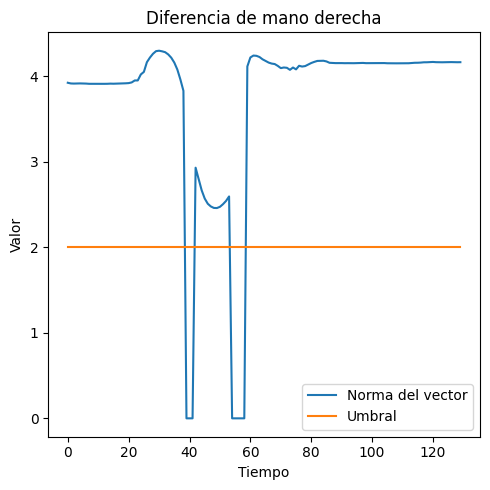
\includegraphics[align=t,width=0.9\linewidth, height =0.9\linewidth]{Graphics/umbral_missing_rhand_aborto}
		\caption{Umbral en la gráfica de la mano derecha del token ``aborto''}
		\label{f:umbral_rhand_aborto}
	\end{subfigure}
	\begin{subfigure}[t]{0.3\textwidth}
		\centering
		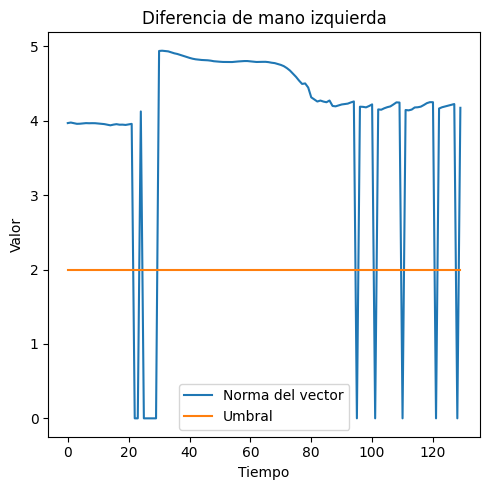
\includegraphics[align=t,width=0.9\linewidth, height =0.9\linewidth]{Graphics/umbral_missing_lhand_aborto}
		\caption{Umbral en la gráfica de la mano izquierda del token ``aborto''}
		\label{f:umbral_lhand_aborto}
	\end{subfigure}
	\begin{subfigure}[t]{0.3\textwidth}
		\centering
		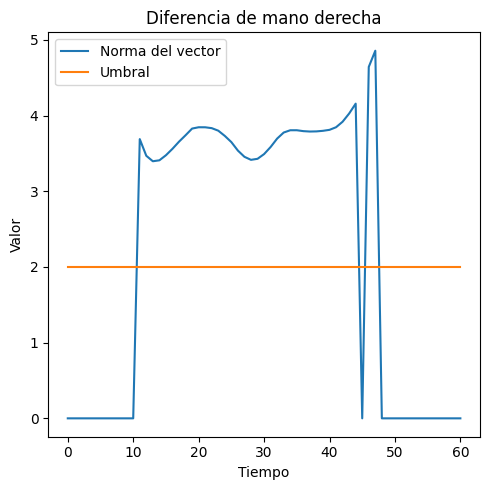
\includegraphics[align=t,width=0.9\linewidth, height =0.9\linewidth]{Graphics/umbral_missing_rhand_amar}
		\caption{Umbral en la gráfica de la mano derecha del token ``amar''}
		\label{f:umbral_rhand_amar}
	\end{subfigure}
	\caption{Umbral de detección de las manos faltantes en los tokens ``aborto'' y ``amar'' Fig \ref{f:manos_faltantes}.}
	\label{f:umbral_deteccion_manos_faltantes}
\end{figure}

Mientras que en la Fig \ref{f:no_manos_faltantes} se puede analizar la comparativa con respecto al token sin normalizar.

Este experimento brindó buenos resultados al realizarse con el método de interpolación lineal, mientras que el cúbico, a pesar de aportar mayor suavidad, en intervalos cortos generaba perturbaciones y alargamiento de extremidades.

\subsection{Experimento 2}
Para este segundo experimento se evalúa la efectividad del recorte por inactividad en un mismo token mediante la verificación de los extremos del mismo y gráficas que cuantifican el movimiento general y por las manos. En cuanto a la Fig \ref{f:recorte_aborto} se puede verificar como el método de recorte por inactividad está detectando los intervalos de mayor cantidad de movimiento. Siendo estos mayoritariamente los del medio de la grabación, ya que en los extremos es que suele estar en reposo el señante. En la Fig \ref{f:fluidez_novariable} se podrá apreciar mejor el recorte puesto que se ve el principio y el final actual de cada token de muestra.


\begin{figure}[t]
\centering
	\begin{subfigure}[t]{0.3\textwidth}
	\centering
		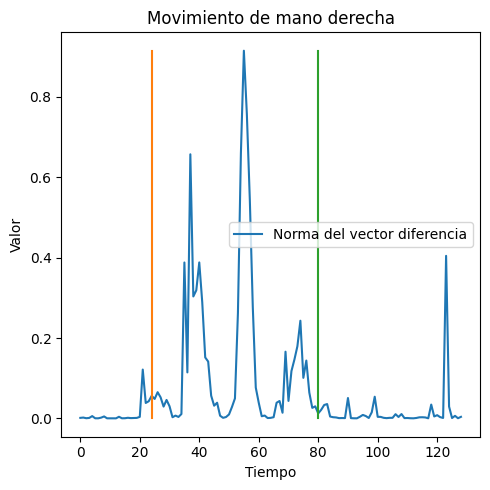
\includegraphics[align=t,width=0.9\linewidth, height =0.9\linewidth]{Graphics/umbrales_recorte_rhand_aborto.png}
		\caption{ Umbrales para recortar del movimiento de la mano derecha del token }
		\label{f:rhand_movediff_amar}
	\end{subfigure}
	\begin{subfigure}[t]{0.3\textwidth}
	\centering
		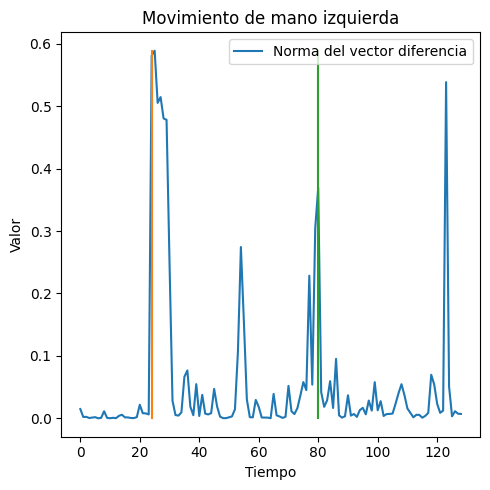
\includegraphics[align=t,width=0.9\linewidth, height =0.9\linewidth]{Graphics/umbrales_recorte_lhand_aborto.png}
		\caption{Umbrales para recortar del movimiento de la mano izquierda del token }
		\label{f:lhand_movediff_amar}
	\end{subfigure}
		\begin{subfigure}[t]{0.3\textwidth}
	\centering
		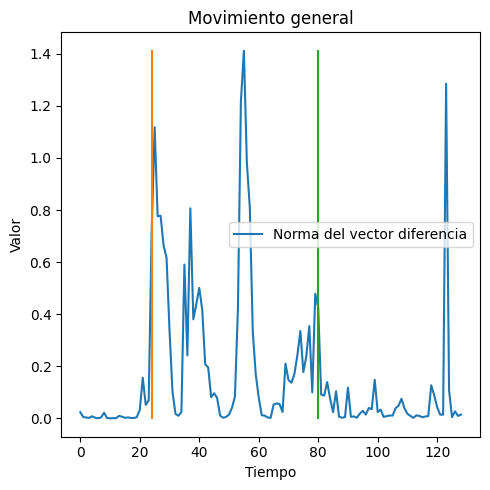
\includegraphics[align=t,width=0.9\linewidth, height =0.9\linewidth]{Graphics/umbrales_recorte_general_aborto.png}
		\caption{Umbrales para recortar del movimiento de la mano derecha del token  }
		\label{f:general_movediff_amar}
	\end{subfigure}
	\vskip 0pt
	\begin{subfigure}[t]{0.3\textwidth}
	\centering
		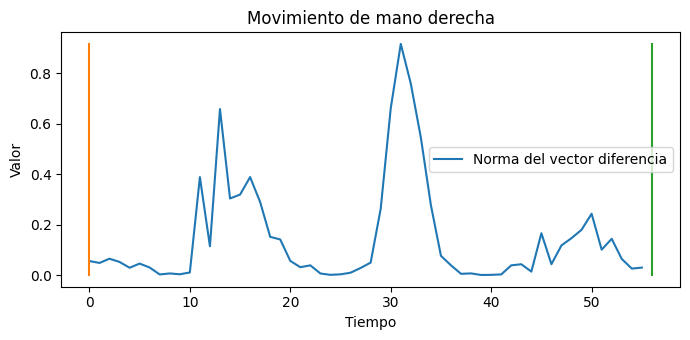
\includegraphics[align=t,width=0.9\linewidth, height =0.9\linewidth]{Graphics/recorte_rhand_aborto.png}
		\caption{Recorte de movimiento de la mano derecha del token  }
		\label{f:rhand_movediff_aborto}
	\end{subfigure}
	\begin{subfigure}[t]{0.3\textwidth}
	\centering
		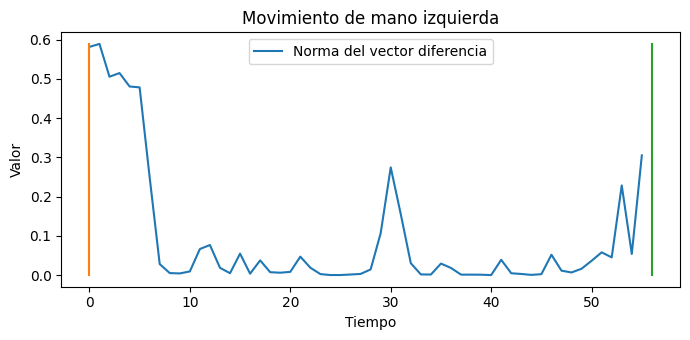
\includegraphics[align=t,width=0.9\linewidth, height=0.9\linewidth]{Graphics/recorte_lhand_aborto.png}
		\caption{Recorte de movimiento de la mano izquierda del token  }
		\label{f:lhand_movediff_aborto}
	\end{subfigure}
	\begin{subfigure}[t]{0.3\textwidth}
	\centering
		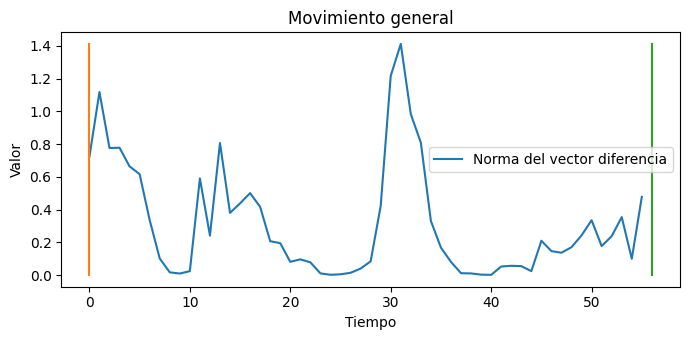
\includegraphics[align=t,width=0.9\linewidth, height=0.9\linewidth]{Graphics/recorte_general_aborto.png}
		\caption{Recorte de movimiento general del token  }
		\label{f:general_movediff_aborto}
	\end{subfigure}
	\caption{Detección de umbrales en las gráficas de movimiento por manos y general del token ``aborto'' normalizado. Véase Fig \ref{f:movediff_aborto_amar}}
	\label{f:recorte_aborto}
\end{figure}

\begin{figure}[t]
\centering
		\begin{subfigure}[t]{0.3\textwidth}
		\centering
		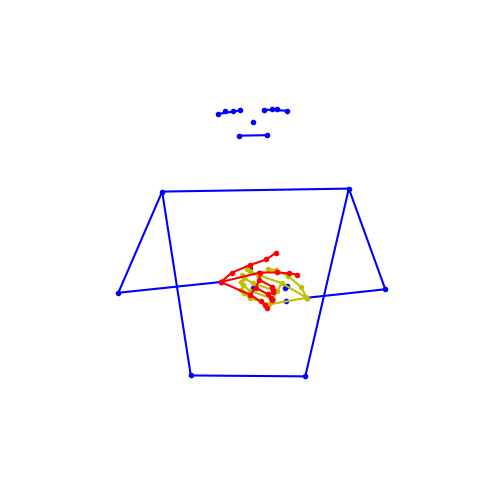
\includegraphics[align=t,width=0.9\linewidth, height =0.9\linewidth]{Graphics/cropped_principio_aborto.png}
		\caption{Principio del token recortado y normalizado ``aborto''}
		\label{f:principio_novariable_aborto}
	\end{subfigure}
		\begin{subfigure}[t]{0.3\textwidth}
		\centering
		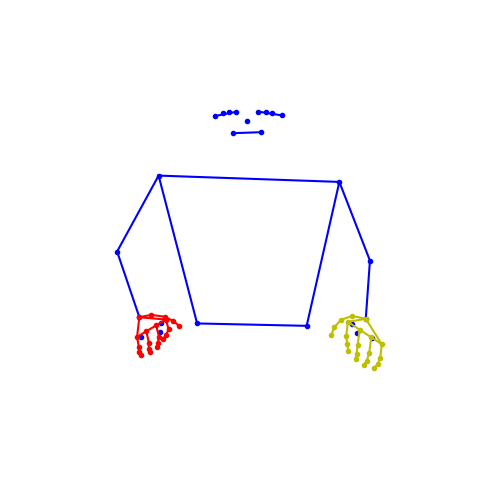
\includegraphics[align=t,width=0.9\linewidth, height =0.9\linewidth]{Graphics/cropped_principio_amar.png}
		\caption{Principio del token recortado y normalizado ``amar''}
		\label{f:principio_novariable_amar}
	\end{subfigure}	
	\vskip 0pt
	\begin{subfigure}[t]{0.3\textwidth}
		\centering
		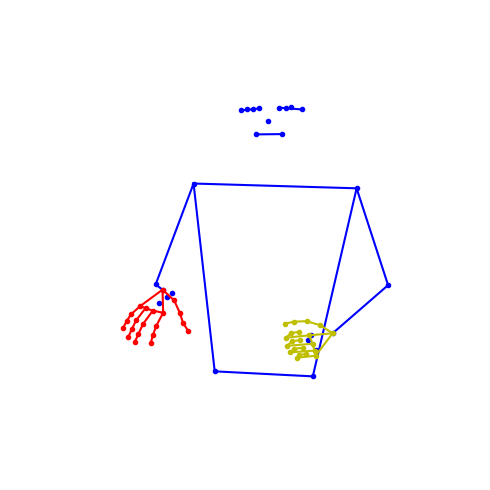
\includegraphics[align=t,width=0.9\linewidth, height =0.9\linewidth]{Graphics/cropped_final_aborto.png}
		\caption{Final del token recortado y normalizado ``aborto''}
		\label{f:final_novariable_aborto}
	\end{subfigure}
	\begin{subfigure}[t]{0.3\textwidth}
		\centering
		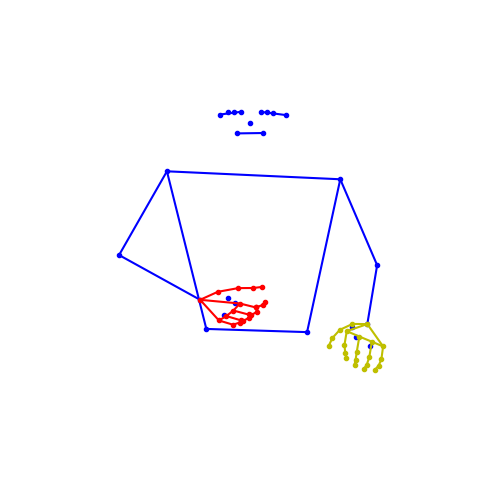
\includegraphics[align=t,width=0.9\linewidth, height =0.9\linewidth]{Graphics/cropped_final_amar.png}
		\caption{Final del token recortado y normalizado ``amar''}
		\label{f:final_novariable_amar}
	\end{subfigure}
	
	\caption{Resultados obtenidos en cuanto a diferencias mostradas en la Fig \ref{f:fluidez_variable}.}
	\label{f:fluidez_novariable}
\end{figure}

Este experimento demostró excelentes resultados, jugando un papel especial el hecho de escoger de manera efectiva las funciones que cuantifican el movimiento, la función a maximizar y el porcentaje de movimiento total a mantener. Valores distintos a los escogidos por defecto pueden devenir en exceso de recorte o ninguno.

\subsection{Experimento 3}
Para este tercer experimento se decide valorar el correcto posicionamiento y ajuste de la mano falsa, así como la interpolación en la suma entre dos tokens. Para ello se eligen al token al correspondiente a la seña de aborto y de la seña amar, puesto que este último carece de manos en ambos extremos en su token original sin normalizar ni realizarle recorte por inactividad. Se evaluó de positivo el uso de las manos falsas y la interpolación interna para solucionar el problema de las manos faltantes como se ve en la Fig \ref{f:no_manos_faltantes}.

\begin{figure}[t]
\centering
		\begin{subfigure}[t]{0.3\textwidth}
		\centering
		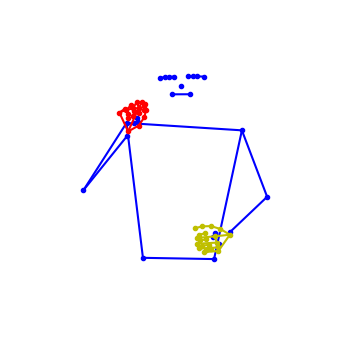
\includegraphics[align=t,width=0.9\linewidth, height =0.9\linewidth]{Graphics/mano_antes_desaparecer}
		\caption{Mano antes de desaparecer del token original ``aborto''}
		\label{f:no_mano_faltante_0}
	\end{subfigure}
	\hskip 0pt
	\begin{subfigure}[t]{0.3\textwidth}
		\centering
		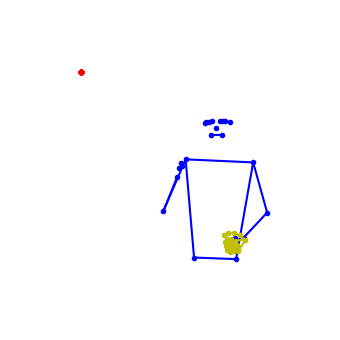
\includegraphics[align=t,width=0.9\linewidth, height =0.9\linewidth]{Graphics/mano_desaparecida}
		\caption{Frame siguiente al anterior del token original ``aborto''}
		\label{f:no_mano_faltante_1}
	\end{subfigure}
		\vskip 0pt
		\begin{subfigure}[t]{0.3\textwidth}
		\centering
		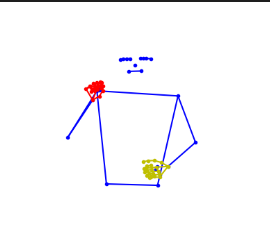
\includegraphics[align=t,width=0.9\linewidth, height =0.9\linewidth]{Graphics/anterior_a_missing_hand_aborto}
		\caption{Mano antes de, supuestamente, desaparecer del token recortado y normalizado ``aborto''}
		\label{f:no_mano_faltante_0}
	\end{subfigure}
	\hskip 0pt
	\begin{subfigure}[t]{0.3\textwidth}
		\centering
		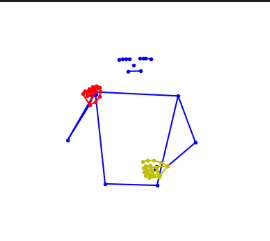
\includegraphics[align=t,width=0.9\linewidth, height =0.9\linewidth]{Graphics/ya_no_missing_hand_aborto}
		\caption{Frame siguiente al anterior del token recortado y normalizado ``aborto''}
		\label{f:no_mano_faltante_1}
	\end{subfigure}
	
	
	\caption{Resultados obtenidos en cuanto a diferencias mostradas en la Fig \ref{f:manos_faltantes}.}
	\label{f:no_manos_faltantes}
	\end{figure}
	
Además, uno de los mejores resultados obtenidos durante la experimentación fue la secuencia de interpolación entre 2 señas con finales tan marcados [véase la Fig \ref{f:seq_interpol} para una mejor apreciación].
	\begin{figure}[t]
\centering
	\begin{subfigure}[t]{0.3\textwidth}
	\centering
		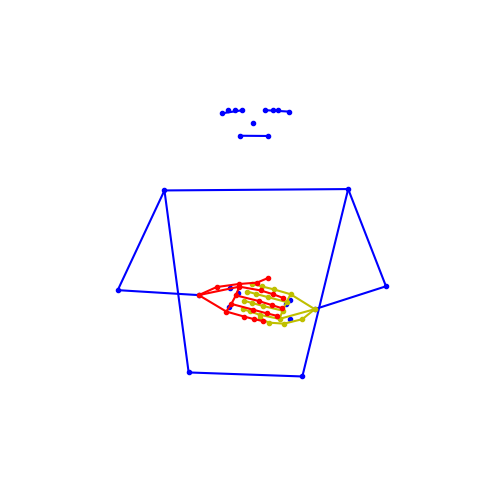
\includegraphics[align=t,width=0.9\linewidth, height =0.9\linewidth]{Graphics/interpol_aborto_amar_0.png}
		\caption{ Frame 0}
		\label{f:frame0}
	\end{subfigure}
	\begin{subfigure}[t]{0.3\textwidth}
	\centering
		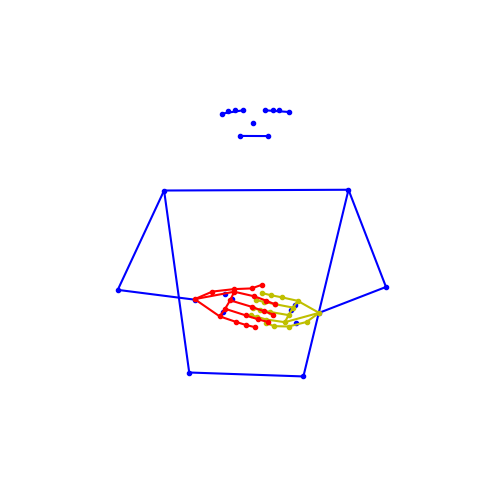
\includegraphics[align=t,width=0.9\linewidth, height =0.9\linewidth]{Graphics/interpol_aborto_amar_1.png}
		\caption{Frame 1 }
		\label{f:frame1}
	\end{subfigure}
	\begin{subfigure}[t]{0.3\textwidth}
	\centering
		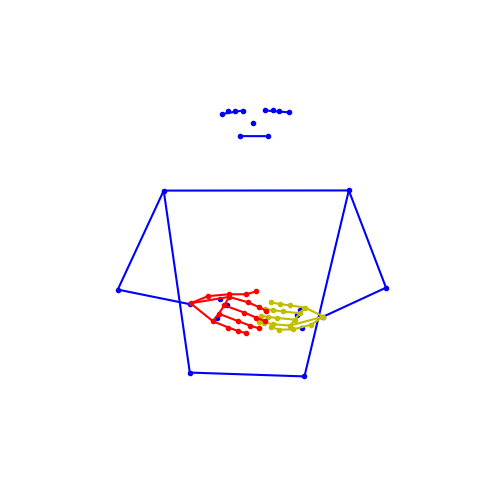
\includegraphics[align=t,width=0.9\linewidth, height =0.9\linewidth]{Graphics/interpol_aborto_amar_2.png}
		\caption{Frame 2 }
		\label{f:frame2}
	\end{subfigure}
	\vskip 0pt
	\begin{subfigure}[t]{0.3\textwidth}
		\centering
		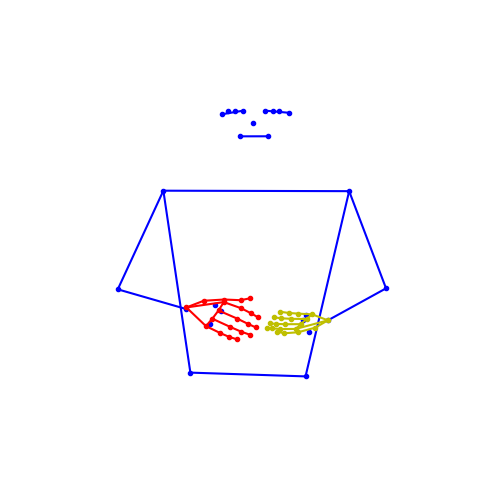
\includegraphics[align=t,width=0.9\linewidth, height =0.9\linewidth]{Graphics/interpol_aborto_amar_3.png}
		\caption{Frame 3}
		\label{f:frame3}
	\end{subfigure}
	\begin{subfigure}[t]{0.3\textwidth}
		\centering
		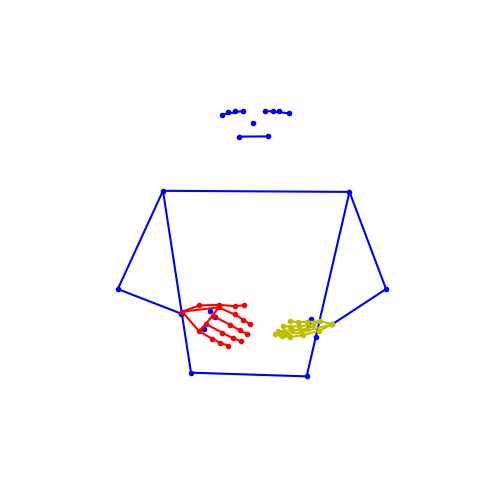
\includegraphics[align=t,width=0.9\linewidth, height =0.9\linewidth]{Graphics/interpol_aborto_amar_4.png}
		\caption{Frame 4 }
		\label{f:frame4}
	\end{subfigure}
	\begin{subfigure}[t]{0.3\textwidth}
		\centering
		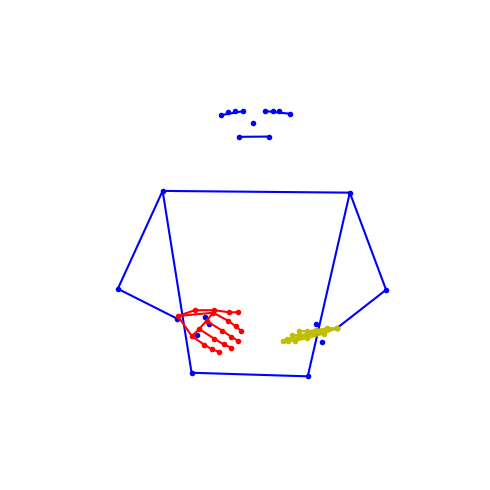
\includegraphics[align=t,width=0.9\linewidth, height =0.9\linewidth]{Graphics/interpol_aborto_amar_5.png}
		\caption{Frame 5 }
		\label{f:frame5}
	\end{subfigure}
	\vskip 0pt
	\begin{subfigure}[t]{0.3\textwidth}
	\centering
		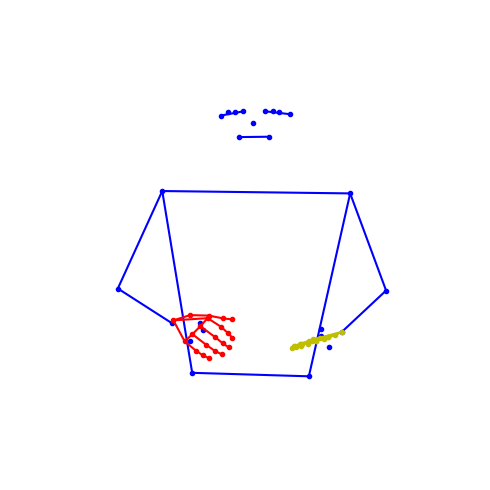
\includegraphics[align=t,width=0.9\linewidth, height=0.9\linewidth]{Graphics/interpol_aborto_amar_6.png}
		\caption{Frame 6}
		\label{f:frame6}
	\end{subfigure}
	\begin{subfigure}[t]{0.3\textwidth}
	\centering
		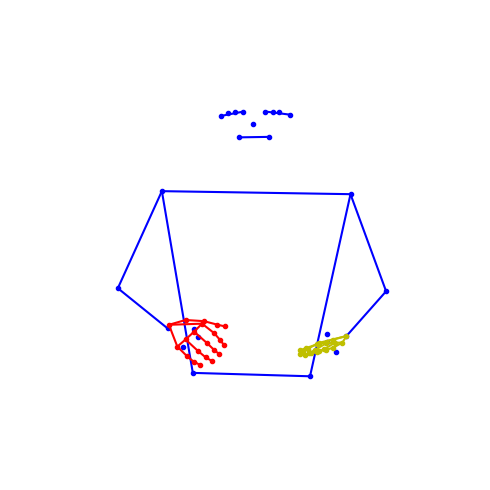
\includegraphics[align=t,width=0.9\linewidth, height=0.9\linewidth]{Graphics/interpol_aborto_amar_7.png}
		\caption{Frame 7}
		\label{f:frame7}
	\end{subfigure}
	\begin{subfigure}[t]{0.3\textwidth}
	\centering
		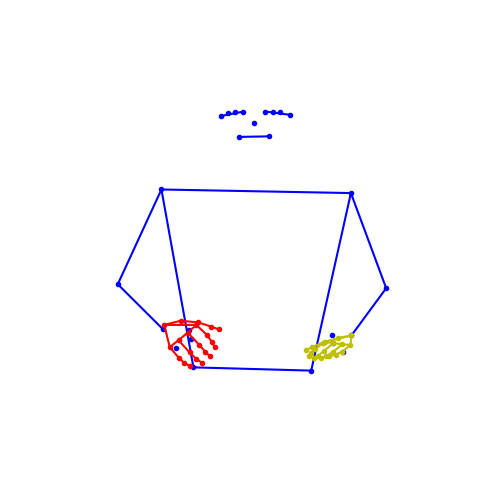
\includegraphics[align=t,width=0.9\linewidth, height =0.9\linewidth]{Graphics/interpol_aborto_amar_8.png}
		\caption{Frame 8}
		\label{f:frame8}
	\end{subfigure}
	\vskip 0pt
	\begin{subfigure}[t]{0.3\textwidth}
	\centering
		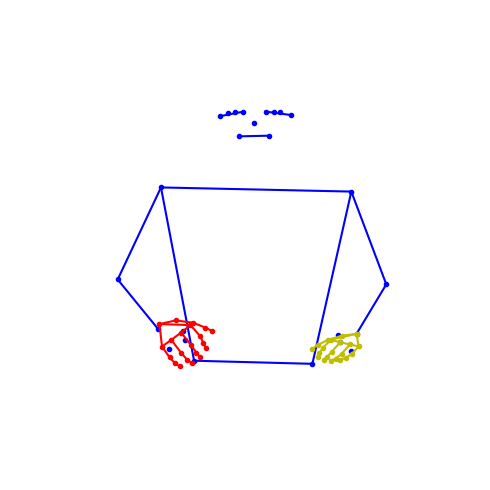
\includegraphics[align=t,width=0.9\linewidth, height =0.9\linewidth]{Graphics/interpol_aborto_amar_9.png}
		\caption{Frame 9}
		\label{f:frame9}
	\end{subfigure}
	\begin{subfigure}[t]{0.3\textwidth}
	\centering
		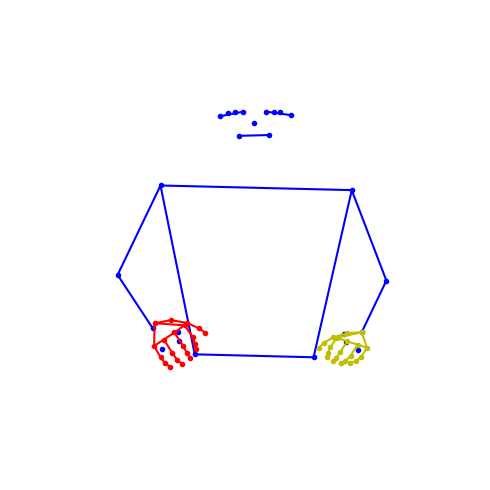
\includegraphics[align=t,width=0.9\linewidth, height =0.9\linewidth]{Graphics/interpol_aborto_amar_10.png}
		\caption{Frame 10}
		\label{f:frame10}
	\end{subfigure}
	\begin{subfigure}[t]{0.3\textwidth}
	\centering
		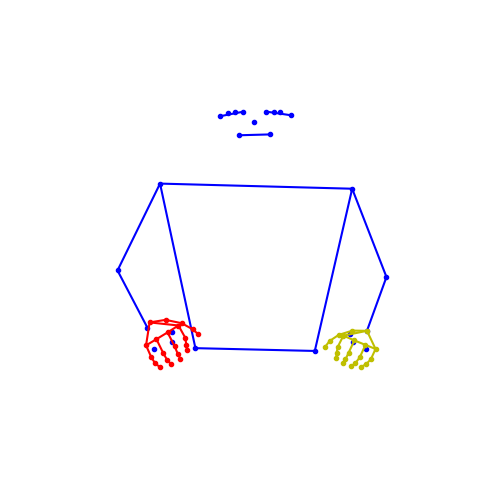
\includegraphics[align=t,width=0.9\linewidth, height =0.9\linewidth]{Graphics/interpol_aborto_amar_11.png}
		\caption{Frame 11 }
		\label{f:frame11}
	\end{subfigure}
	\caption{Secuencia Interpolada entre el token ``aborto'' y ``amar''. Véase Fig \ref{f:fluidez_novariable} para notar los extremos a unirse.}
	\label{f:seq_interpol}
\end{figure}
Este experimento se comportó de manera correcta, a pesar de que la mano no corresponde con la original o presenta una disposición diferente a la que originalmente perteneciera a la imagen. Dado que no existe una referencia en la imagen original se puede evaluar como positivo el desempeño demostrado.
\subsection{Experimento 4}
Se decidió probar si la solución presentada para exportar a formato BVH era al menos una aproximación inicial. Para ello se evaluó de manera perceptual la secuencia generada por el archivo BVH importándolo a la aplicación del motor gráfico Blender




\begin{figure}[t]
\centering
		\begin{subfigure}[t]{0.3\textwidth}
		\centering
		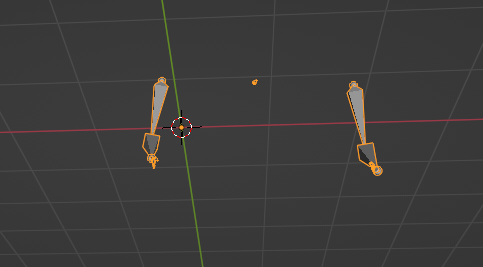
\includegraphics[align=t,width=0.9\linewidth, height =0.9\linewidth]{Graphics/blender_bvh_1.png}
		\caption{Frame 0}
		\label{f:bframe0}
	\end{subfigure}
		\begin{subfigure}[t]{0.3\textwidth}
		\centering
		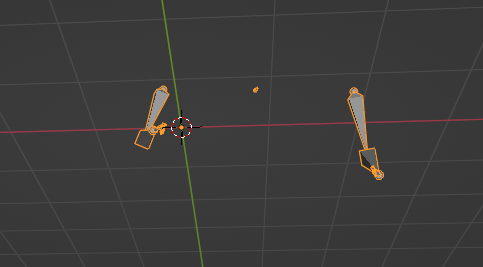
\includegraphics[align=t,width=0.9\linewidth, height =0.9\linewidth]{Graphics/blender_bvh_2.png}
		\caption{Frame 1}
		\label{f:bframe1}
	\end{subfigure}	
	\vskip 0pt
	\begin{subfigure}[t]{0.3\textwidth}
		\centering
		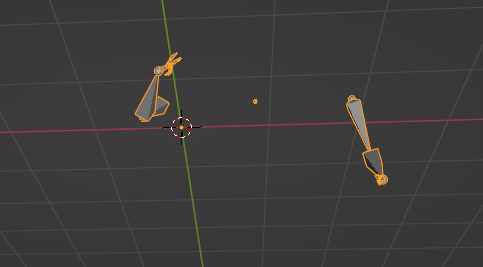
\includegraphics[align=t,width=0.9\linewidth, height =0.9\linewidth]{Graphics/blender_bvh_3.png}
		\caption{Frame 2}
		\label{f:bframe2}
	\end{subfigure}
	\begin{subfigure}[t]{0.3\textwidth}
		\centering
		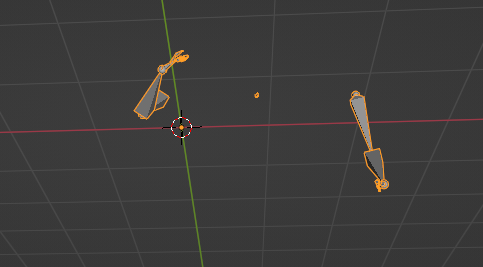
\includegraphics[align=t,width=0.9\linewidth, height =0.9\linewidth]{Graphics/blender_bvh_4.png}
		\caption{Frame 3}
		\label{f:bframe3}
	\end{subfigure}
	
	\caption{Resultado del archivo BVH del token recortado y normalizado ``amar''}
	\label{f:amar_bvh}
\end{figure}
Los resultados obtenidos con la generación de un archivo BVH no fueron aceptables. Por desconocimiento de algunos de los ángulos de rotación y como definirlos correctamente, solo se pudo armar el esqueleto pero su movilidad deja mucho que desear. Muchas de las uniones no pueden moverse en algunas direcciones a pesar de que hace el intento por replicar la seña de la cual fue hecho [véase Fig \ref{f:amar_bvh}].

\section{Discusión}

A partir de los experimentos realizados se pudo concluir que la propuesta brindó buenos resultados fuera del ámbito de la animación. Muchos factores como bibliotecas de python como bpy (Módulo de Blender para Python) que no llegaron a instalarse nunca podrían haber acelerado o incluso hacer muy ligero y transparente el proceso de llevar el \textit{TokenLSC} a BVH e incluso a animación 3D.
Pese a los buenos resultados en todos los demás aspectos, aún quedan estructuras y proporciones en las que trabajar, dado que la forma del cuerpo, así como su proporción, dependen mucho de factores como:
\begin{itemize}
\item ángulo de inclinación de la grabación
\item estructura corporal del señante
\item fallos en el modelo de reconocimiento
\end{itemize}
La solución implementada brinda generalización y extensibilidad para su uso en otros fines tanto para generar nuevo contenido audiovisual como para registrar nuevas señas al conjunto de datos.




